\documentclass[11pt]{article}

\usepackage[utf8]{inputenc}
\usepackage[T1]{fontenc}
\usepackage{geometry}
\usepackage{booktabs}
\usepackage{graphicx}
\usepackage{amsmath}
\usepackage{longtable}
\usepackage{array}
\usepackage{float}
\usepackage{lscape}
\usepackage{tikz}
\usetikzlibrary{shapes,arrows,positioning,decorations.pathreplacing}
\usepackage{listings}
\usepackage{xcolor}

% Page setup
\geometry{margin=1in}
\setlength{\parskip}{6pt plus 2pt minus 1pt}
\setlength{\parindent}{0pt}

\begin{document}

% Header information
{\Large\bfseries Semiconductor Analysis}

\textbf{Joshua Gao}\\[0.3em]
Private Equity Investment Analysis\\[0.3em]
Yale University\\[0.3em]
\today\\[0.5em]

\textit{In this report, I analyze five companies: NVIDIA (NVDA), Intel (INTC), Advanced Micro Devices (AMD), Microchip Technology (MCHP), and Lattice Semiconductor (LSCC). Each company is a major player in the semiconductor industry, providing computing devices for a wide range of applications, from training artificial intelligence models to powering desktop computers. Several of these companies also sell software and other related services to their end customers. The predominant return drivers for these companies stem from four key elements of the factor value chain: product slate, operational efficiency (ROI on R\&D spending), capitalization, and multiple (market expectations for growth with AI). In the comparables analysis section of this report, I analyze each of these four elements in detail across the five companies. Then, in the acquisition analysis section, I propose a potential acquisition of Lattice Semiconductor by NVIDIA.}

\section{Comparables}
\subsection{Product Slate}
The semiconductor industry produces computing chips that densely compact transistors and various electronic elements onto silicon wafers. A key fact is that the specific arrangement of transistors and electronic elements on these wafers can vary greatly, each having very different end use cases (product slate differentiation) and requiring different business strategies to distribute. An overview of each product and the associated business product slate is provided in Table \ref{tab:1}.

\begin{table}[H]
\centering
\caption{Company Overview and Market Position}
\label{tab:1}
\footnotesize
\setlength{\tabcolsep}{5pt}
\renewcommand{\arraystretch}{1.1}
\resizebox{\textwidth}{!}{%
\begin{tabular}{lllrrr}
\toprule
Ticker & Company Name & Primary Focus & Revenue (\$B) & Market Cap (\$B) & 3-Yr CAGR (\%) \\
\midrule
NVDA & NVIDIA Corporation & Graphics Processing Units (GPUs) & \$130.5 & \$4,387.8 & 115.85\% \\
INTC & Intel Corporation & Central Processing Units (CPUs) & \$53.1 & \$190.8 & -20.20\% \\
AMD & Advanced Micro Devices Inc. & CPUs and GPUs & \$25.8 & \$357.8 & 18.37\% \\
MCHP & Microchip Technology Inc. & Microcontrollers, Memory Chips & \$4.4 & \$28.9 & -17.98\% \\
LSCC & Lattice Semiconductor Corp. & Field-Programmable Gate Arrays (FPGAs) & \$0.5 & \$9.4 & -7.56\% \\
\bottomrule
\end{tabular}%
}
\end{table}



At the low unit-price end of the spectrum are MCUs (microcontrollers) and ASICs (application-specific integrated circuits) produced by MCHP. These are often implemented in small consumer devices, and the price per chip has been driven down through competition to \$0.03 to \$0.50 per unit. Thus, to justify the R\&D costs behind developing these chipsets, massive volume is needed. Running this business is fundamentally different from the business of other chipmakers. MCHP is sensitive to commodity pricing, and their product, being hardware, only has limited ability to be replaced and continuously resold to customers. Thus, they are heavily sensitive to operational inefficiencies and changes in input costs to chip-making. 

In the middle are FPGAs, which are a type of ASIC that can be programmed after manufacturing to be used in a wide range of applications. FPGAs are distinct in that they solve problems for low-volume buyers that need the specification and tunability of ASICs, but their particular use case does not justify high-volume development of these chip forms in MCUs, while at the same time needing something more specialized, cost-effective, and specifically optimized for performance than GPUs. This positioning makes FPGAs particularly valuable for edge computing applications, where customization and low power consumption are critical.

At the high cost end are GPUs, which can often be in the \$10,000 range. These high-performance chips are essential for AI training and inference, data center operations, and high-end graphics rendering. The premium pricing reflects both the complexity of the chips and the strong demand from AI applications.


\subsection{Multiple (Market Expectations for Growth with AI)}
Each product solves problems for its own market segment, and each market segment has its own expectations for growth. NVDA stands out among this group with the highest market capitalization of \$4.4 trillion: it began as a company specialized in building GPUs for computer graphic visualization. Then, as AI capabilities became more promising, demand for NVDA's chips greatly increased as people needed a way to quickly train new models. NVDA's product slate has not changed significantly (other than incremental improvements every year), but the expectations (multiple of the factor value chain) for growth have skyrocketed. NVIDIA trades at 33.62x revenue, reflecting the market's extraordinary expectations for continued AI-driven growth. 

Other companies, on the other hand, have a more modest market cap to revenue multiple, ranging from 3.59x for Intel (INTC) to 18.45x for Lattice Semiconductor (LSCC), with Advanced Micro Devices (AMD) at 13.88x and Microchip Technology (MCHP) at 6.57x. Lattice Semiconductor's high multiple is due to its unique position in the industry, specializing in FPGAs. The growth expectations reflected in these valuation multiples are further supported by revenue CAGR data: NVDA leads with a remarkable 115.85\% three-year CAGR, followed by AMD at 18.37\%, while INTC shows declining revenue with a -20.20\% CAGR, reflecting the challenges facing mature CPU manufacturers.

\begin{table}[H]
\centering
\caption{Valuation Multiples - Market Expectations}
\footnotesize
\setlength{\tabcolsep}{4pt}
\renewcommand{\arraystretch}{0.9}
\resizebox{\textwidth}{!}{%
\begin{tabular}{l@{\hspace{30pt}}rrrrrr}
\toprule
Company & Mkt Cap/Rev & EV/Rev & P/B & P/CF & P/E & EV/EBITDA \\
 & (x) & (x) & (x) & (x) & (x) & (x) \\
\midrule
NVDA & 33.62 & 32.58 & 36.78 & 63.5 & 60.0 & 47.2 \\
INTC & 3.59 & 4.13 & 1.79 & 179.7 & N/A & N/A \\
AMD & 13.88 & 13.60 & 5.89 & 164.6 & 218.0 & 129.2 \\
MCHP & 6.57 & 7.75 & 4.31 & 722.5 & N/A & 134.8 \\
LSCC & 18.45 & 18.65 & 13.28 & 136.7 & 153.5 & 373.6 \\
\midrule
\multicolumn{7}{l}{\footnotesize\textit{Mkt Cap/Rev \& P/CF are most relevant for growth expectations.}} \\
\multicolumn{7}{l}{\footnotesize\textit{EV/EBITDA is misleading in some cases (e.g., LSCC 373.6x = \$25M EBITDA vs \$9.5B EV).}} \\
\bottomrule
\end{tabular}%
}
\end{table}

\textit{Note: Companies with negative earnings (INTC and MCHP) show "N/A" for some metrics. Financial data is from the most recent annual 10-K filings. Market data is as of December 2025.}

\subsection{Operational Efficiency (ROI on R\&D spending)}
As the baseline for technology advances, each company aims to improve their offerings within the industry and must continuously iterate on their product slate. This requires significant R\&D spending, which is reflected in the operating margins of each company. Gross margins range from NVDA at the top, able to command high prices on GPUs given strong demand (chips are often sold out) at 78.4\%, to INTC at the bottom at 25.3\%. NVDA is able to maintain these high gross margins down to an operating margin of 66.0\%, while AMD's operating margin is 7.5\% and INTC's operating margin is -5.3\%. Other companies have lower operating margins. These low operating margins can be explained by increased spending on research and development, with LSCC's low operating margin of 2.0\% explained by its highest R\&D spending of 31.1\% of revenue. INTC is heavily investing in R\&D (\$16.5 billion, representing 31.1\% of revenue) to improve its chip manufacturing processes to maintain its market share, despite facing declining revenue growth. The differences in operational efficiency reflect how effectively each company converts R\&D spending into profitable operations, with NVDA demonstrating superior ability to maintain high margins despite significant R\&D investments, while companies like LSCC and INTC show lower operating margins due to their high R\&D intensity relative to their revenue base.

\begin{table}[H]
\centering
\caption{R\&D Intensity and Profitability Margins}
\footnotesize
\setlength{\tabcolsep}{6pt}
\renewcommand{\arraystretch}{1.1}
\resizebox{\textwidth}{!}{%
\begin{tabular}{llllll}
\toprule
Company & Gross Margin (\%) & Operating Margin (\%) & R\&D/Revenue (\%) & R\&D Spending (\$B) \\
\midrule
NVDA & 78.4\% & 66.0\% & 8.0\% & \$10.4 \\
INTC & 25.3\% & -5.3\% & 31.1\% & \$16.5 \\
AMD & 44.9\% & 7.5\% & 26.0\% & \$6.7 \\
MCHP & 27.6\% & 2.7\% & 18.0\% & \$0.8 \\
LSCC & 50.5\% & 2.0\% & 31.1\% & \$0.2 \\
\bottomrule
\end{tabular}%
}
\end{table}



\subsection{Capitalization}
The capitalization structure of each company reflects its stage in the industry lifecycle and strategic priorities. INTC and MCHP are the most highly levered companies in the group, with debt-to-equity ratios of 97.9\% and 117.2\% respectively, compared to NVDA's 40.7\% and AMD's 20.3\%. These are also the companies that have been around for the longest and have reached greater maturity in their respective technologies, with their pricing showing lower expectations for growth. Both companies are struggling with margins: INTC's operating margin of -5.3\% and net margin of -35.3\% reflect significant profitability challenges, while MCHP's operating margin of 2.7\% and essentially break-even net margin (-0.01\%) demonstrate thin profitability despite its 27.6\% gross margin. MCHP similarly maintains high leverage while operating in the mature microcontroller and memory chip markets. 

The capitalization structure reflects each company's stage in the industry lifecycle: mature companies like INTC and MCHP rely more heavily on debt financing, while growth companies like NVDA and AMD maintain lower leverage ratios, preserving financial flexibility for strategic investments and acquisitions. This financial flexibility is particularly important for NVDA, which has used its strong balance sheet to make strategic acquisitions and invest heavily in R\&D to maintain its competitive position in the AI chip market.

\begin{table}[H]
\centering
\caption{Capitalization Structure and Leverage}
\tiny
\setlength{\tabcolsep}{6pt}
\renewcommand{\arraystretch}{1.1}
\resizebox{\textwidth}{!}{%
\begin{tabular}{llllll}
\toprule
Company & Debt/Equity (\%) & Debt/Assets (\%) & Current Ratio (x) \\
\midrule
NVDA & 40.7\% & 28.9\% & 4.44 \\
INTC & 97.9\% & 49.5\% & 1.33 \\
AMD & 20.3\% & 16.8\% & 2.62 \\
MCHP & 117.2\% & 54.0\% & 2.59 \\
LSCC & 19.0\% & 15.8\% & 3.66 \\
\bottomrule
\end{tabular}%
}
\end{table}



The following tables provide detailed financial metrics for each company, including market performance, revenue and profitability analysis, operating metrics, and growth trends.

\begin{table}[H]
\centering
\caption{Comprehensive Comparable Companies Analysis}
\setlength{\tabcolsep}{20pt}
\renewcommand{\arraystretch}{0.85}
\resizebox{\textwidth}{!}{%
\begin{tabular}{lrrrrr}
\toprule
\textbf{Metric} & \textbf{NVDA} & \textbf{INTC} & \textbf{AMD} & \textbf{MCHP} & \textbf{LSCC} \\
\midrule
\multicolumn{6}{l}{\textit{\textbf{Market Performance}}} \\
\midrule
Stock Price (\$) & 179.92 & 40.01 & 219.76 & 53.43 & 68.61 \\
Market Cap (\$B) & 4,387.8 & 190.8 & 357.8 & 28.9 & 9.4 \\
Enterprise Value (\$B) & 4,251.3 & 219.4 & 350.8 & 34.1 & 9.5 \\
\midrule
\multicolumn{6}{l}{\textit{\textbf{Revenue \& Profitability}} (\$M unless noted)} \\
\midrule
Revenue & 130,497 & 53,101 & 25,785 & 4,402 & 509 \\
Gross Profit & 102,370 & 13,432 & 11,575 & 1,215 & 257 \\
Gross Margin (\%) & 78.4 & 25.3 & 44.9 & 27.6 & 50.5 \\
Operating Income & 86,088 & -2,794 & 1,942 & 121 & 10 \\
Operating Margin (\%) & 66.0 & -5.3 & 7.5 & 2.7 & 2.0 \\
EBITDA & 96,528 & 1,454 & 4,005 & 473 & 51 \\
EBITDA Margin (\%) & 74.0 & 2.7 & 15.5 & 10.7 & 10.0 \\
Net Income & 72,880 & -18,756 & 1,641 & -0.5 & 61 \\
Net Margin (\%) & 55.8 & -35.3 & 6.4 & -0.01 & 12.0 \\
ROE (\%) & 91.9 & -18.9 & 2.9 & -0.01 & 8.6 \\
ROA (\%) & 65.3 & -9.5 & 2.4 & -0.00 & 7.2 \\
\midrule
\multicolumn{6}{l}{\textit{\textbf{Cash Flow}} (\$M)} \\
\midrule
Operating CF & 69,115 & 1,062 & 2,173 & 40 & 69 \\
Free CF & 57,371 & -3,717 & -148 & -86 & 23 \\
\midrule
\multicolumn{6}{l}{\textit{\textbf{Operating Metrics}}} \\
\midrule
R\&D/Revenue (\%) & 8.0 & 31.1 & 26.0 & 18.0 & 31.1 \\
Asset Turnover (x) & 1.17 & 0.27 & 0.37 & 0.29 & 0.60 \\
Current Ratio (x) & 4.44 & 1.33 & 2.62 & 2.59 & 3.66 \\
Debt/Equity (x) & 0.41 & 0.98 & 0.20 & 1.17 & 0.19 \\
Debt/Assets (\%) & 28.92 & 49.48 & 16.84 & 53.96 & 15.76 \\
\midrule
\multicolumn{6}{l}{\textit{\textbf{Growth \& Per-Share}}} \\
\midrule
3-Yr CAGR (\%) & 115.85 & -20.20 & 18.37 & -17.98 & -7.56 \\
EPS (\$) & 3.00 & -3.93 & 1.01 & -0.00 & 0.45 \\
BV/Share (\$) & 3.26 & 20.81 & 35.36 & 13.10 & 5.20 \\
\midrule
\multicolumn{6}{l}{\textit{\textbf{Valuation Multiples}} (x)} \\
\midrule
Mkt Cap/Rev & 33.62 & 3.59 & 13.88 & 6.57 & 18.45 \\
EV/Revenue & 32.58 & 4.13 & 13.60 & 7.75 & 18.66 \\
EV/EBITDA & 44.04 & 150.92 & 87.59 & 72.14 & 186.80 \\
EV/EBIT & 49.38 & N/A & 180.63 & 282.09 & 937.11 \\
P/E & 60.0 & N/A & 218.0 & N/A & 153.5 \\
P/B & 36.78 & 1.79 & 5.89 & 4.31 & 13.28 \\
\midrule
\multicolumn{6}{l}{\footnotesize\textit{Note: P/E = Market Cap / Net Income. N/A for negative earnings.}} \\
\multicolumn{6}{l}{\footnotesize\textit{Data from 10-K filings, market data as of Dec 2025.}} \\
\bottomrule
\end{tabular}%
}
\end{table}




\noindent\textit{Note: Over the semester I had the chance to experiment more with using AI tools. I built a pipeline to directly patch into EDGAR SEC's public database to pull data straight from 10-K filings. The above tables are bare financial metrics collected from filings. I then wrote code in Python to calculate all ratios and metrics. This approach of using AI to write code avoids the hallucinations that can come from AI-generated data.}

\newpage

\section{Acquisition}
Having analyzed the comparables across the four key elements of the factor value chain, I now turn to a potential acquisition opportunity. The analysis above reveals that while NVDA dominates in GPUs and AI applications, LSCC occupies a unique position in the FPGA market with strong gross margins but constrained operating margins due to high R\&D intensity. This creates an opportunity for NVDA to diversify its business while providing Lattice with the financial resources needed to accelerate growth. Below, I will walk through the staging framework process, focusing on (1) leadership, (2) economics, (3) context, (4) unmitigated risks, (5) drivers (analyzed above in comparables section). Then I will complete the steps of the frameworks in the process section where the deal process is outlined: covering the (6) exit, (7) transaction probability, (8) price, and (9) returns of the transaction.

\subsection{Leadership}
NVDA's management team, led by CEO Jensen Huang, has demonstrated exceptional execution in capitalizing on AI trends and maintaining operational discipline. Lattice's leadership brings deep expertise in FPGA technology and relationships with customers in edge computing, IoT, and industrial applications. NVDA is headquartered in Santa Clara, California, while Lattice is headquartered in San Jose, California. In an acquisition, it would be important to retain key technical talent to preserve the FPGA business's specialized knowledge and customer relationships, while leveraging NVDA's broader resources and market reach. 

\subsection{Economics, Context, and Risks}
NVDA's historical performance has been closely linked to expectations for AI. For example, earlier this year, when DeepSeek announced a method to train LLMs with minimal compute, NVDA stock dropped 17\% in one day. This volatility demonstrates NVDA's exposure to AI market sentiment. To hedge against this risk, NVDA may want to diversify its business into other areas. Additionally, NVDA's talent density and advanced manufacturing capabilities may create synergies with other chip companies. As investors are waiting for positive unit economics for AI, the overall industry may be at an inflection point where adjustments in expectations may be due.

In recent years, significant focus from academic research institutions has been invested in FPGA research and development. These chips are increasingly seen as critical components for edge AI applications, where low power consumption and programmability are essential. The growing demand for customizable computing solutions in 5G infrastructure, autonomous vehicles, and IoT devices positions FPGAs as a strategic growth area within the semiconductor industry. 

I propose an acquisition of Lattice by NVDA to gain access to the FPGA market. NVDA's market cap is \$4.39 trillion, while Lattice's market cap is \$9.39 billion—NVDA is approximately 467 times larger. However, more importantly for deal financing, NVDA holds \$60.61 billion in cash, which provides 6.5 times coverage of Lattice's current market capitalization, giving NVDA ample financial capacity to execute an all-cash transaction.

The two companies are vastly different in size, but both are financially healthy with positive net income: NVDA reported net income of \$72.9 billion, while Lattice reported \$61 million. Gross margins for these products are both high, with NVDA at 78.4\% and Lattice at 50.5\%. However, Lattice appears to be operationally intensive, with an operating margin of 2.0\% compared to NVDA's 66.0\%. This difference is largely explained by Lattice's R\&D spending, which represents approximately 31\% of revenue, compared to NVDA's R\&D spending of approximately 8\% of revenue. NVDA, being the buyer, has comfortable financials to propose a tender offer for Lattice. Lattice may not be inclined to accept a share swap given the risk associated with NVDA stock price being valued largely based on expectations. This, in addition to the fact that NVDA has substantial cash reserves, suggests that the optimal deal structure would be an all-cash transaction.

This analysis would be incomplete without mentioning several reasons this transaction may not be ideal. NVDA may want to focus on the software side of the business, expanding its data center offerings and purely betting on AI plays. Key risks include: (1) integration challenges, as FPGA businesses require different go-to-market strategies and sales channels than NVDA's current GPU-focused business model; (2) potential distraction from NVDA's core AI business; (3) the capital-intensive nature of FPGA R\&D may not align with NVDA shareholders' expectations for capital efficiency; and (4) regulatory scrutiny, as NVDA's size and market position may attract antitrust concerns. However, the strategic benefits of diversification and access to the growing FPGA market may outweigh these risks. 

\subsection{Process}
For NVDA to execute this transaction, the company would pursue a long-form friendly acquisition with Lattice, initiating it with a tender offer for Lattice's stock. The process would unfold as follows. NVDA would need to enter privileged negotiations with Lattice. Lattice might authorize senior executives to conduct these initial conversations, and eventually, as the conversations progress, Lattice's board would establish a Special Committee to officially oversee the process. These conversations, to NVDA's advantage, would preferably be confidential, as other companies in the sector (e.g., AMD or INTC) may also be interested in acquiring Lattice simultaneously.

One might believe that NVDA, with large cash reserves, should undergo a two-step acquisition procedure to achieve a faster deal close, increasing the transaction probability. However, while NVDA could attempt to gain a controlling proportion of shares, they would need to win two-thirds supermajority (66.67\%) support of the shareholders to approve any significant transaction (as outlined in Article VIII of Lattice's articles of incorporation). Thus, the truly more likely process, which can be executed with a Lattice 50\% board vote, is the friendly process. A friendly acquisition also reduces integration risk and preserves key relationships with Lattice's customers and employees.

Should the board of Lattice accept the tender offer, the deal would enter the next stage of the process. Both the board and shareholders would need to approve the deal. The deal would then be finalized, and the companies would merge. The merged company would be a major player in the semiconductor industry, with a market cap of \$4.4 trillion and combined revenue of approximately \$131 billion (NVDA's \$130.5 billion plus Lattice's \$0.5 billion). The merged company would maintain NVDA's strong gross margin of 78.4\% and operating margin of 66.0\%, with the FPGA business contributing additional revenue streams. The merged company would have a debt-to-equity ratio of approximately 28.9\% and a return on equity of 91.9\%, reflecting NVDA's continued financial strength while adding strategic diversification through FPGA capabilities. At this point, there will be significant responsibility from leadership to think about how to integrate both companies well. Special consideration might be given to the culture, goals, and mission of the combined organization, to ensure that workers are clear with their roles and responsibilities and can produce effective output.

\subsection{Price and Returns (Has-Gets)}
To arrive at how this transaction might be priced, I first analyze what the synergies between NVDA and Lattice might be to understand NVDA's expectations for growth, which will inform how the transaction is priced. Rather than focusing on cash flow returns (which are negative given the premium paid), I assess whether synergies can boost Lattice's revenue enough to justify the \$12.2B transaction value when valued at its current 18.45x revenue multiple. Table \ref{tab:revenue_synergy} shows how different synergy scenarios translate to revenue increases and corresponding valuation boosts. Value creation is defined as the difference between this boosted valuation and the \$12.2B transaction value. The probability-weighted expected value of \$123.1M is what is used in the Has-Gets analysis. Notice that the expectation in immediate value creation is negative, meaning that even at the expected synergy level, the transaction does not create value when valued using Lattice's current market multiple. This is because the transaction premium is 30\%, and the expected synergy is 24.2\%. For NVDA to engage in this transaction, there must be an increase in the multiple for NVDA as well, which is fundamentally the return driver for the deal – that diversification of NVDA's efforts into the FPGA market will increase expected growth.

Expected returns for NVDA could come from several sources: (1) revenue synergies from cross-selling FPGA solutions to NVDA's existing customer base; (2) cost synergies from combining R\&D operations and leveraging NVDA's manufacturing scale; (3) strategic value from diversification away from pure AI exposure; and (4) access to the growing FPGA market, particularly in edge AI applications.
\begin{table}[H]
\centering
\caption{Value Creation from Revenue Synergies}
\label{tab:revenue_synergy}
\footnotesize
\setlength{\tabcolsep}{4pt}
\renewcommand{\arraystretch}{1.0}
\resizebox{\textwidth}{!}{%
\begin{tabular}{lrrrrrr}
\toprule
Scenario & Revenue & Revenue & Valuation & Value & Success & Prob \\
& Synergy & Increase & @ 18.45x & Creation & Metric & (\%) \\
& (\$M) & (\%) & (\$B) & (\$B) & (\%) & \\
\midrule
Very Pessimistic & \$15.0M & 2.9\% & \$9.68B & \$-2.53B & -20.7\% & 5\% \\
Pessimistic & \$37.0M & 7.3\% & \$10.08B & \$-2.12B & -17.4\% & 7\% \\
Base Case & \$73.9M & 14.5\% & \$10.76B & \$-1.44B & -11.8\% & 13\% \\
Base & \$123.2M & 24.2\% & \$11.67B & \$-0.53B & -4.3\% & 38\% \\
Optimistic & \$160.2M & 31.4\% & \$12.35B & \$0.15B & 1.3\% & 25\% \\
Bull Case & \$184.8M & 36.3\% & \$12.81B & \$0.61B & 5.0\% & 9\% \\
Very Bull & \$221.8M & 43.5\% & \$13.49B & \$1.29B & 10.6\% & 3\% \\
\midrule
\textbf{Expected Value} & \textbf{\$123.1M} & \textbf{24.2\%} & \textbf{\$11.67B} & \textbf{\$-0.53B} & \textbf{-4.4\%} & \textbf{100\%} \\
\bottomrule
\end{tabular}%
}
\begin{flushleft}
\scriptsize
\textit{Note: Revenue synergies match the \$123.2M annual synergies from Has-Gets analysis. Valuation uses Lattice\textquotesingle s current revenue multiple of 18.45x. Value Creation = New Valuation - Transaction Value (\$12.2B). Success Metric = Value Creation as \% of Transaction Value. Probabilities sum to 100\% and are normally distributed with Base case (\$123.2M) at 38\% probability. Expected value of \$123.1M matches Has-Gets base synergies.}
\end{flushleft}
\end{table}


In the Has-Gets analysis, I propose an all-cash transaction at \$89.19 per share, representing a 30\% premium over Lattice's current market price of \$68.61. The total transaction value would be approximately \$12.2 billion, well within NVDA's financial capacity given its \$60.61 billion cash position.
\begin{table}[H]
\centering
\caption{Has-Gets Analysis: NVIDIA Acquisition of Lattice Semiconductor}
\label{tab:hasgets}
\setlength{\tabcolsep}{6pt}
\renewcommand{\arraystretch}{0.85}
\resizebox{\textwidth}{!}{%
\begin{tabular}{lrrrr}
\toprule
Metric & \multicolumn{2}{c}{Seller (LSCC)} & Buyer Has & Buyer Gets \\
\cmidrule(lr){2-3}
& Has & Gets & (NVDA) & (All Cash, With Synergies) \\
\midrule
\multicolumn{5}{l}{\textit{Valuation Metrics}} \\
\midrule
Share price (\$) & 68.61 & 89.19 & 179.92 & 179.92 \\
P/E ratio (x) & 153.5 & N/A & 60.0 & 60.1 \\
Market cap (\$B) & 9.39 & 12.20 & 4,387.8 & 4,387.8 \\
\midrule
\multicolumn{5}{l}{\textit{Credit Ratios}} \\
\midrule
Debt/EBITDA (x) & 5.23 & N/A & 0.33 & 0.36 \\
EBITDA/Interest (x) & 4.78 & N/A & 69.7 & 69.6 \\
Debt/Capitalization (\%) & 15.8 & N/A & 28.9 & 28.8 \\
Net Debt/Capitalization (\%) & 1.8 & N/A & -25.4 & -14.3 \\
\midrule
\multicolumn{5}{l}{\textit{Balance Sheet Items}} \\
\midrule
Total Debt (\$B) & 0.13 & -- & 32.27 & 32.41 \\
Cash \& Equivalents (\$B) & 0.12 & 12.20 & 60.61 & 48.53 \\
Net Debt (\$B) & 0.02 & -12.20 & -28.34 & -16.12 \\
Equity (\$B) & 0.71 & -- & 79.33 & 78.62 \\
\midrule
\multicolumn{5}{l}{\textit{Income Statement (Pro Forma)}} \\
\midrule
Revenue (\$B) & 0.51 & N/A & 130.50 & 131.13 \\
EBITDA (\$B) & 0.03 & N/A & 96.53 & 96.68 \\
Net Income (\$B) & 0.06 & N/A & 72.88 & 73.04 \\
\midrule
\multicolumn{5}{l}{\textit{Transaction Details}} \\
\midrule
Offer Price per Share (\$) & -- & 89.19 & -- & -- \\
Premium to Market (\%) & -- & 30.0 & -- & -- \\
Total Consideration (\$B) & -- & 12.20 & -- & -- \\
Goodwill Created (\$B) & -- & -- & -- & 11.49 \\
\bottomrule
\end{tabular}%
}
\begin{flushleft}
\scriptsize
\textit{Note: Seller Gets reflects cash consideration at \$89.19/share (30\% premium). Cash \& Equivalents shows \$12.20B received. Operating metrics (P/E, credit ratios, income statement) are N/A as Lattice shareholders receive cash and company ceases to exist. Buyer Gets shows pro forma combined entity. Synergies assume \$123.2M annual (after-tax \$97.3M). All-cash transaction structure.}
\end{flushleft}
\end{table}



As a sanity check, for context on the valuation premium, historical semiconductor M\&A transactions provide context for valuation and deal structure. The transaction multiples (EV/Revenue, EV/EBITDA, P/E) vary significantly based on target characteristics, growth prospects, and strategic fit. Premiums ranging from 11.9\% to 57.0\%, with my proposed 30\% premium falling within the typical range.
\begin{table}[H]
\centering
\caption{Comparable Transaction Multiples - Semiconductor M\&A}
\label{tab:comps}
\footnotesize
\setlength{\tabcolsep}{3pt}
\renewcommand{\arraystretch}{0.95}
\resizebox{\textwidth}{!}{%
\begin{tabular}{llllrrrr}
\toprule
Acquirer & Target & Date & Transaction Value & Premium & EV/Revenue & EV/EBITDA & P/E \\
 &  &  & (\$M) & (\%) & (x) & (x) & (x) \\
\midrule
AMD & Xilinx & 2022 & \$49,000 & 24.8\% & 15.8x & 54.4x & 75.4x \\
Analog Devices & Maxim Integrated & 2021 & \$20,900 & 22.0\% & 9.1x & 27.9x & 36.7x \\
Marvell Technology & Inphi & 2020 & \$10,000 & 57.0\% & 20.0x & 83.3x & 222.2x \\
Intel & Mobileye & 2017 & \$15,300 & 34.0\% & 42.7x & 153.0x & 204.0x \\
Broadcom & CA Technologies & 2018 & \$18,900 & 20.0\% & 4.5x & 17.2x & 22.2x \\
NXP Semiconductors & Freescale Semiconductor & 2015 & \$11,800 & 11.9\% & 2.6x & 8.4x & 23.6x \\
\midrule
\textit{Mean} & & & & \textit{28.1\%} & \textit{15.6x} & \textit{57.4x} & \textit{97.5x} \\
\textit{Median} & & & & \textit{23.4\%} & \textit{12.4x} & \textit{40.9x} & \textit{55.5x} \\
\midrule
\multicolumn{8}{l}{\footnotesize\textit{Source: Public company filings and press releases. Premiums calculated as \% over target's 30-day average stock price prior to announcement.}} \\
\bottomrule
\end{tabular}%
}
\end{table}


\input{./ma/ma_analysis}

\newpage
\section*{Appendix: Project Structure and Coding Pipeline}

\subsection*{File Structure}

\begin{center}
\resizebox{0.95\textwidth}{!}{%
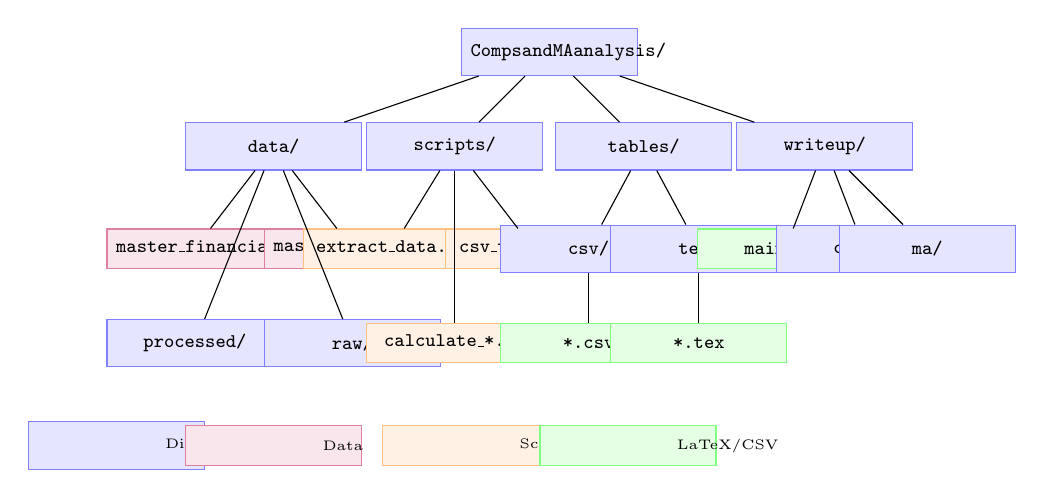
\begin{tikzpicture}[
    every node/.style={font=\scriptsize},
    dir/.style={rectangle, draw=blue!50, fill=blue!10, minimum width=2cm, minimum height=0.6cm, text width=2cm, align=center},
    file/.style={rectangle, draw=green!50, fill=green!10, minimum width=2cm, minimum height=0.5cm, text width=2cm, align=center},
    script/.style={rectangle, draw=orange!50, fill=orange!10, minimum width=2cm, minimum height=0.5cm, text width=2cm, align=center},
    data/.style={rectangle, draw=purple!50, fill=purple!10, minimum width=2cm, minimum height=0.5cm, text width=2cm, align=center}
]
    % Root
    \node[dir] (root) at (0,0) {\texttt{CompsandMAanalysis/}};
    
    % Level 1 directories
    \node[dir] (data) at (-3.5,-1.2) {\texttt{data/}};
    \node[dir] (scripts) at (-1.2,-1.2) {\texttt{scripts/}};
    \node[dir] (tables) at (1.2,-1.2) {\texttt{tables/}};
    \node[dir] (writeup) at (3.5,-1.2) {\texttt{writeup/}};
    
    % Data subdirectories
    \node[data] (master) at (-4.5,-2.5) {\texttt{master\_financials.json}};
    \node[data] (comps) at (-2.5,-2.5) {\texttt{master\_comps.csv}};
    \node[dir] (processed) at (-4.5,-3.7) {\texttt{processed/}};
    \node[dir] (raw) at (-2.5,-3.7) {\texttt{raw/}};
    
    % Scripts files
    \node[script] (extract) at (-2,-2.5) {\texttt{extract\_data.py}};
    \node[script] (csvtex) at (-0.2,-2.5) {\texttt{csv\_to\_latex.py}};
    \node[script] (ratios) at (-1.2,-3.7) {\texttt{calculate\_*.py}};
    
    % Tables subdirectories
    \node[dir] (csv) at (0.5,-2.5) {\texttt{csv/}};
    \node[dir] (tex) at (1.9,-2.5) {\texttt{tex/}};
    \node[file] (csvfiles) at (0.5,-3.7) {\texttt{*.csv}};
    \node[file] (texfiles) at (1.9,-3.7) {\texttt{*.tex}};
    
    % Writeup files
    \node[file] (maintex) at (3,-2.5) {\texttt{main.tex}};
    \node[dir] (compsdir) at (4,-2.5) {\texttt{comps/}};
    \node[dir] (madir) at (4.8,-2.5) {\texttt{ma/}};
    
    % Connections
    \draw (root) -- (data);
    \draw (root) -- (scripts);
    \draw (root) -- (tables);
    \draw (root) -- (writeup);
    
    \draw (data) -- (master);
    \draw (data) -- (comps);
    \draw (data) -- (processed);
    \draw (data) -- (raw);
    
    \draw (scripts) -- (extract);
    \draw (scripts) -- (csvtex);
    \draw (scripts) -- (ratios);
    
    \draw (tables) -- (csv);
    \draw (tables) -- (tex);
    \draw (csv) -- (csvfiles);
    \draw (tex) -- (texfiles);
    
    \draw (writeup) -- (maintex);
    \draw (writeup) -- (compsdir);
    \draw (writeup) -- (madir);
    
    % Legend
    \node[dir] (legdir) at (-5.5,-5) {};
    \node[anchor=west, font=\tiny] at (-5,-5) {Directory};
    \node[data] (legdata) at (-3.5,-5) {};
    \node[anchor=west, font=\tiny] at (-3,-5) {Data};
    \node[script] (legscript) at (-1,-5) {};
    \node[anchor=west, font=\tiny] at (-0.5,-5) {Script};
    \node[file] (legfile) at (1,-5) {};
    \node[anchor=west, font=\tiny] at (1.5,-5) {LaTeX/CSV};
\end{tikzpicture}%
}
\end{center}

\subsection*{Coding Pipeline}

\begin{center}
\resizebox{0.95\textwidth}{!}{%
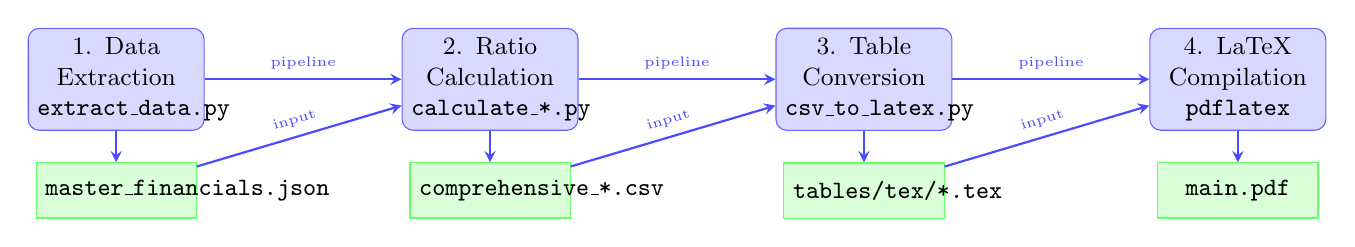
\begin{tikzpicture}[
    node distance=1.2cm,
    every node/.style={font=\small},
    process/.style={rectangle, draw=blue!60, fill=blue!15, minimum width=2.2cm, minimum height=1cm, text width=2cm, text centered, rounded corners},
    data/.style={rectangle, draw=green!60, fill=green!15, minimum width=1.8cm, minimum height=0.7cm, text width=1.8cm, text centered},
    arrow/.style={->, >=stealth, thick, blue!70}
]
    % Step 1
    \node[process] (step1) at (0,0) {1. Data\\Extraction\\\texttt{extract\_data.py}};
    \node[data, below=0.4cm of step1] (data1) {\texttt{master\_financials.json}};
    \draw[arrow] (step1) -- (data1);
    
    % Step 2
    \node[process, right=2.5cm of step1] (step2) {2. Ratio\\Calculation\\\texttt{calculate\_*.py}};
    \node[data, below=0.4cm of step2] (data2) {\texttt{comprehensive\_*.csv}};
    \draw[arrow] (step2) -- (data2);
    \draw[arrow] (data1) -- node[above, font=\tiny, sloped] {input} (step2);
    
    % Step 3
    \node[process, right=2.5cm of step2] (step3) {3. Table\\Conversion\\\texttt{csv\_to\_latex.py}};
    \node[data, below=0.4cm of step3] (data3) {\texttt{tables/tex/*.tex}};
    \draw[arrow] (step3) -- (data3);
    \draw[arrow] (data2) -- node[above, font=\tiny, sloped] {input} (step3);
    
    % Step 4
    \node[process, right=2.5cm of step3] (step4) {4. LaTeX\\Compilation\\\texttt{pdflatex}};
    \node[data, below=0.4cm of step4] (data4) {\texttt{main.pdf}};
    \draw[arrow] (step4) -- (data4);
    \draw[arrow] (data3) -- node[above, font=\tiny, sloped] {input} (step4);
    
    % Flow arrows
    \draw[arrow] (step1) -- node[above, font=\tiny] {pipeline} (step2);
    \draw[arrow] (step2) -- node[above, font=\tiny] {pipeline} (step3);
    \draw[arrow] (step3) -- node[above, font=\tiny] {pipeline} (step4);
\end{tikzpicture}%
}
\end{center}

\vspace{0.5cm}

\textbf{Key Pipeline Components:}

\begin{itemize}
    \item \textbf{Data Extraction}: Python scripts connect directly to SEC EDGAR's public database using the \texttt{edgartools} library to extract financial data from 10-K filings. This ensures data accuracy by pulling directly from source documents rather than relying on potentially outdated third-party databases.
    
    \item \textbf{Automated Calculations}: All financial ratios, metrics, and M\&A analysis calculations (CAGR, IRR sensitivity, revenue synergies, Has-Gets analysis) are computed programmatically in Python. This approach eliminates manual calculation errors and ensures consistency across all metrics.
    
    \item \textbf{Table Generation}: CSV files are automatically converted to LaTeX table format, maintaining consistent formatting across all tables in the document. Tables can be edited in CSV format (using Excel or similar tools) and then regenerated as LaTeX.
    
    \item \textbf{Version Control}: All data extractions are timestamped and saved to \texttt{data/processed/}, allowing for reproducibility and historical tracking of data versions.
\end{itemize}

\textit{This pipeline leverages AI tools to write code that extracts and processes data, avoiding the hallucinations that can occur when AI generates financial data directly. The code ensures accuracy by pulling from authoritative sources (SEC filings) and performing transparent, verifiable calculations.}

\end{document}